\documentclass[11pt, openright]{book}

    % Cover Variables
    \newcommand{\ctoptitle}{}
    \newcommand{\ctitle}{Title}
    \newcommand{\cautor}{Author}
    \newcommand{\cdate}{day.month.year}
    \newcommand{\sectittle}{Second Title}


    % Header Variables
        \newcommand{\headRE}{Main Topic}
        \newcommand{\headLE}{\emph{\rightmark}}
        \newcommand{\footRE}{Lucas Lescure $-$ \cdate}
        \newcommand{\footLE}{\emph{\thepage}}

    % TOC Variables
        \newcommand{\toctitle}{Table of Content}
        
        \newcommand{\tocchapter}{Chapter}
        \newcommand{\toccount}{3}
  
    % Chapter Variables
        \newcommand{\chvar}{Chapter -}

\usepackage[a4paper, total={16cm, 22.125cm}]{geometry}

% Page Style
\usepackage[]{environ}
% Cover Page 
\usepackage{tikz}
\makeatletter
\def\parsecomma#1,#2\endparsecomma{\def\page@x{#1}\def\page@y{#2}}
\tikzdeclarecoordinatesystem{page}{
    \parsecomma#1\endparsecomma
    \pgfpointanchor{current page}{north east}
    % Save the upper right corner
    \pgf@xc=\pgf@x%
    \pgf@yc=\pgf@y%
    % save the lower left corner
    \pgfpointanchor{current page}{south west}
    \pgf@xb=\pgf@x%
    \pgf@yb=\pgf@y%
    % Transform to the correct placement
    \pgfmathparse{(\pgf@xc-\pgf@xb)/2.*\page@x+(\pgf@xc+\pgf@xb)/2.}
    \expandafter\pgf@x\expandafter=\pgfmathresult pt
    \pgfmathparse{(\pgf@yc-\pgf@yb)/2.*\page@y+(\pgf@yc+\pgf@yb)/2.}
    \expandafter\pgf@y\expandafter=\pgfmathresult pt
}
\makeatother


% Object formatting
\usepackage[12pt]{moresize}
\usepackage[]{anyfontsize}
\usepackage{titlesec}
\usepackage{import}
\usepackage{floatrow}
\usepackage{enumitem}
\usepackage{changepage}
\usepackage[normalem]{ulem}
\usepackage{array}
\newcommand{\ul}[1]{\underline{#1}}

\usepackage[]{chngcntr}
\usepackage{ifthen}
\ifthenelse{\figcountdepth > 1}
  {\counterwithin{figure}{section}\counterwithin{table}{section}}
  {}

\usepackage[format=plain, labelfont=it, textfont=it]{caption}
\makeatletter
\def\@makecaption#1#2{%
    \vskip\abovecaptionskip
    \sbox\@tempboxa{\textit{#1.} #2}

       
   

    \ifdim \wd\@tempboxa >\hsize
        #1. #2\par
    \else
        \global \@minipagefalse
        \hb@xt@\hsize{\hfil\box\@tempboxa\hfil}
    \fi
    \vskip\belowcaptionskip}
\makeatother

\DeclareCaptionFormat{underline}{\uline{#1#2#3}\par}

% Sections
\titleformat{\section}{\fontsize{16}{19.2}\bfseries}{\thesection.}{0.25em}{}
\titleformat{\subsection}{\fontsize{14}{16.8}\bfseries}{\tab\thesubsection.}{0.25em}{}
\titleformat{\subsubsection}{\fontsize{10}{12}}{\uline{\thesubsubsection)\enspace}}{0em}{\uline}





% Geometry

% Typewritting

\setlength{\parskip}{1em}
\setlength{\parindent}{0em}


\newenvironment{items}[3][0pt]
{\def\closesep{#3}
    \vspace{#2}
    \begin{itemize}
        \setlength{\itemsep}{#1}
        \setlength{\topsep}{0pt}
        \setlength{\partopsep}{0pt}}
        {\end{itemize}
    \vspace{\closesep}}

\newenvironment{enum}[3][0pt]
{\defclosesep{#3}
    \vspace{#2}
    \begin{enumerate}
        \setlength{\itemsep}{#1}
        \setlength{\topsep}{0pt}
        \setlength{\partopsep}{0pt}}
        {\end{enumerate}
    \vspace{\closesep}}

\newenvironment{eq}[2]
{\def\closesep{#2}
    \vspace{#1}
    \begin{align*}}
        {\end{align*}
    \vspace{\closesep}}

\newenvironment{lfeq}[2]
{\def\closesep{#2}
    \vspace{#1}
    \begin{flalign*}}
        {\end{flalign*}
    \vspace{\closesep}}
% List Formatting


\NewEnviron{dent}[1]{
    \vspace{-10pt}
    \begin{adjustwidth}{7mm}{}
        \uline{#1}\hspace{2mm}
        \BODY
    \end{adjustwidth}
    \vspace{-10pt}
}


\usepackage[framemethod=tikz]{mdframed}
\newcounter{count_theorem}[section]\setcounter{count_theorem}{0}
\newcommand{\thetheorem}{\arabic{count_theorem}}

\newcounter{count_exercise}[section]\setcounter{count_exercise}{0}
\newcommand{\theexercise}{\arabic{count_exercise}}


\newenvironment{theorem}[1][]{
    \refstepcounter{count_theorem}
    \mdfsetup{
        linecolor=red!30,
        innerbottommargin=10pt,
        linewidth=2pt,
        topline=false,
        bottomline=false,
        rightline=false,
        shadow=true,
        shadowsize=4.5pt,
        frametitlerule=false,
        apptotikzsetting={
                \tikzset{
                    mdfbackground/.append style={
                            left color=red!8,right color=red!3
                        }
                }
            }
    }
    \begin{mdframed}[]\relax
        \ifstrempty{#1}
        {\textbf{Theorem~\thetheorem.} }
        {\textbf{Theorem~\thetheorem.~#1} }
        }
        {\end{mdframed}\vspace{-10pt}
}

\newenvironment{note}{
    \mdfsetup{innertopmargin=5pt,
        linecolor=gray!30,
        linewidth=2pt,
        topline=false,
        bottomline=false,
        rightline=false,
        frametitleaboveskip=0pt,
        shadow=false,
        shadowsize=4pt,
        frametitlerule=false,
        apptotikzsetting={
                \tikzset{
                    mdfbackground/.append style={
                            left color=gray!8,right color=gray!3
                        }
                }
            }
    }
    \begin{mdframed}[]\relax
        \textbf{Note. }
        }
        {\end{mdframed}\vspace{-10pt}
}

\newenvironment{example}{
    \mdfsetup{innertopmargin=5pt,
        linecolor=green!30,
        linewidth=2pt,
        topline=false,
        bottomline=false,
        rightline=false,
        frametitleaboveskip=0pt,
        shadow=false,
        shadowsize=4pt,
        frametitlerule=false,
        apptotikzsetting={
                \tikzset{
                    mdfbackground/.append style={
                            left color=green!7,right color=green!2
                        },
                    mdfframetitlebackground/.append style={
                            left color=green!7,right color=green!2
                        }
                }
            }
    }
    \begin{mdframed}[]\relax
        \textbf{Example. }
        }
        {\end{mdframed}\vspace{-10pt}
}


\usetikzlibrary{calc,arrows}

\tikzset{
    excursus arrow/.style={%
            line width=2pt,
            draw=gray!40,
            rounded corners=2ex,
        },
    excursus head/.style={
            fill=white,
            font=\bfseries\sffamily,
            text=gray!80,
            anchor=base west,
        },
    excursus line/.style={%
            line width=2pt,
            draw=gray!40,
            rounded corners=2ex,
        }
}

\newenvironment{exercise}[1][]{%
    \refstepcounter{count_exercise}
    \mdfsetup{
        singleextra={
                \path let \p1=(P), \p2=(O) in (\x2,\y1) coordinate (Q);
                \path let \p1=(Q), \p2=(O) in (\x1,{(\y1-\y2)/2}) coordinate (M);
                \path [excursus line] ($(O)+(5em,0ex)$) -| (M) |- ($(Q)+(20em,0ex)$);
                \node [excursus head] at ($(Q)+(2.5em,-0.75pt)$) {\ifstrempty{#1}{Exercise \theexercise}{Exercise \theexercise:~#1}};},
        firstextra={
                \path let \p1=(P), \p2=(O) in (\x2,\y1) coordinate (Q);
                \path [excursus arrow,-to] (O) |- ($(Q)+(12em,0ex)$) .. controls +(0:16em) and +(185:6em) .. ++(23em,2ex);},
        middlelinewidth=2.5em,middlelinecolor=white,
        hidealllines=true,topline=true,
        innertopmargin=0.5ex,
        innerbottommargin=2.5ex,
        innerrightmargin=2pt,
        innerleftmargin=2ex,
        skipabove=0.87\baselineskip,
        skipbelow=0.62\baselineskip,
    }
    \begin{mdframed}[]\relax}
        {\end{mdframed}\vspace{-10pt}
}

% Functions and Data Plotting
\usepackage{subfig,wrapfig,adjustbox,multirow}


% Plotting Style
\usepackage{graphicx,pgfplots}
\usetikzlibrary{arrows}
\usetikzlibrary {patterns,patterns.meta}
\usepgfplotslibrary{fillbetween}
\pgfplotsset{compat=1.18}

\usepgfplotslibrary{units}
% Logarithmic Scale
\pgfplotsset{
    log x ticks with fixed point/.style={
            xticklabel={
                    \pgfkeys{/pgf/fpu=true}
                    \pgfmathparse{exp(\tick)}%
                    \pgfmathprintnumber[fixed relative, precision=3]{\pgfmathresult}
                    \pgfkeys{/pgf/fpu=false}
                }
        }
}


\input{/root/.config/latex-utils/common/math.tex}

% Headings  
\usepackage[Glenn]{fncychap}
\ChNumVar{\fontsize{40}{42}}
\ChTitleVar{\Large\sc}
\ChNameVar{\Large\sc}
\setlength\headheight{14.5pt}
\renewcommand\FmN[1]{\chvar}



\usepackage{fancyhdr}
\usepackage{ragged2e}

% Header & Footers
\renewcommand{\chaptermark}[1]{\markboth{#1}{#1}}
\renewcommand{\sectionmark}[1]{
    \markright{ #1}
}
\pagestyle{fancy}
\fancyhf{}
\fancyhead[LE,RO]{\headLE}
\fancyhead[RE,LO]{\headRE}
\fancyfoot[LE,RO]{\footLE}
\fancyfoot[RE,LO]{\footRE}
\renewcommand{\headrulewidth}{0.5pt}
\fancyheadoffset{1cm}

\fancypagestyle{plain}{%
    \fancyhf{} % clear all header and footer fields
    \fancyfoot[LE, RO]{\footLE}
    \renewcommand{\headrulewidth}{0pt}
    \renewcommand{\footrulewidth}{0pt}}


\fancypagestyle{nohead}{%
    \fancyhf{} % clear all header 
    \fancyfoot[LE, RO]{\footLE}
    \fancyfoot[LO, RE]{\footRE}}

    \fancypagestyle{head}{%
    \fancyhf{} % clear all header 
    \fancyhead[LE,RO]{\headLE}
\fancyhead[RE,LO]{\headRE}
\renewcommand{\headrulewidth}{0.5pt}
\fancyheadoffset{1cm}
    }


\fancypagestyle{bib}{%
    \fancyhf{} % clear all header and footer fields
    \fancyhead[CE, CO]{}
    \fancyfoot[LE, RO]{\footLE}
    \fancyfoot[LO, RE]{Bibliographie}}

% Table of Contents

\renewcommand*\thechapter{\arabic{chapter}} %Usually Roman
\renewcommand*\thesection{\arabic{section}}
\renewcommand*\thesubsubsection{\thesubsection.\alph{subsubsection}}
\makeatletter
\@removefromreset{section}{chapter}
\makeatother


% Table of Contents

\usepackage{titletoc}
\usepackage[linktoc=all]{hyperref}
\addto{\captionsenglish}{\renewcommand*{\contentsname}{\toctitle}}

\setcounter{secnumdepth}{3}
\setcounter{tocdepth}{\toccount}

\usepackage[subfigure]{tocloft}
\setlength\cftparskip{0pt}

\usepackage{etoolbox}
\makeatletter
\pretocmd{\chapter}{\addtocontents{toc}{\protect\addvspace{5\p@}}}{}{}
\pretocmd{\section}{\addtocontents{toc}{\protect\addvspace{-10\p@}}}{}{}
\pretocmd{\subsection}{\addtocontents{toc}{\protect\addvspace{1\p@}}}{}{}
\makeatother


% Chapter Style
\titlecontents{chapter}
[11em]
{\bigskip}
{\bfseries\textsc\tocchapter~\textsc\thecontentslabel : \textsc}
{\hspace*{-5.5em}\textbf}
{\titlerule*[1pc]{ }}[\smallskip]

% Section Style
\titlecontents{section}
[3em] % i
{\bigskip\bfseries}
{\fontsize{11}{13.2}\bfseries\uline{\thecontentslabel.\enspace}\uline}
{\hspace*{-4em}\textbf}
{\hspace{-2mm}\uline{\hspace*{\fill}}\hspace{-5pt}\contentspage}

% Subsection Style
\titlecontents{subsection}
[5em] % i
{\smallskip\bfseries}
{\fontsize{10}{12}\bfseries\thecontentslabel.\enspace}
{\hspace*{-4em}}
{\titlerule*[0.5pc]{.}\contentspage}



% Subsubsection Style
\titlecontents{subsubsection}
[7em] % i
{\smallskip}
{\fontsize{10}{12}\thecontentslabel)\enspace}
{\hspace*{-4em}}
{\titlerule*[0.5pc]{.}\contentspage}











    % figure support
    \usepackage{import}
    \usepackage{xifthen}
    \pdfminorversion=7
    \usepackage{pdfpages}
    \usepackage{transparent}
    \newcommand{\incfig}[1]{%
            \def\svgwidth{\columnwidth}
            \import{./figures/}{#1.pdf_tex}
    }

    \pdfsuppresswarningpagegroup=1


\begin{document}
% Spacing
\input{/root/.config/latex-utils/common/begin.tex}

% Cover
% Cover
\definecolor{ccolor1}{RGB}{236,145,143}
\definecolor{ccolor2}{RGB}{131,168,192}
\definecolor{ccolor3}{RGB}{182,227,150}
\definecolor{ccolor4}{RGB}{171,206,145}

\begin{titlepage}

    \newgeometry{top=1cm, width=21cm, bottom=1cm}

    \begin{tikzpicture}[remember picture,overlay,every node/.style={anchor=center}]
        \node[opacity =0.07, inner sep=0pt, anchor=east] at (current page.east){\includegraphics[width=0.5\paperwidth,height=\paperheight]{/home/archlinux/.config/latex-utils/logos/invert1.png}};

        %\node[opacity=0.15, inner sep=0pt, anchor=south west] at (current page.south west){\includegraphics[width=0.5\paperwidth,height=0.5\paperheight]{/home/archlinux/.config/latex-utils/logos/invert2.png}};

        \node[opacity=0.15,inner sep=0pt, anchor=north west] at (current page.north west){\includegraphics[width=0.5\paperwidth,height=0.5\paperheight]{/home/archlinux/.config/latex-utils/logos/invert3.png}};

        \node at (page cs:0,0.925) {\LARGE\bfseries\textsc{Telecom Saint-Étienne}};


        %\node[opacity=0.15, inner sep=0pt, anchor=south west] at (current page.south west){\includegraphics[width=0.5\paperwidth,height=0.5\paperheight]{/home/archlinux/.config/latex-utils/logos/invert2.png}};

        \node at (page cs:0,0.6) {\fontsize{28}{28.8}\textbf{\ctoptitle}};
        \node at (page cs:0,0.525) {\fontsize{28}{28.8}\textbf{\ctitle}};
        \draw (page cs:0.5,0.475) -- (page cs:-0.5,0.475);
        \node at (page cs:0,0.445) {\Large\textsc{}};
        \node at (page cs:0,0.4) {\Large\textsc{\cdate}};
        \node[anchor=east] at (page cs:-0.3,0.315) {\Large\textsc{Lucas Lescure: }};
        \node[anchor=west] at (page cs:-0.3,0.335) {\Large\textsc{lucas.lescure1@gmail.com}};
        \node[anchor=west] at (page cs:-0.3,0.295) {\large\textsc{+33 6 16 06 04 45 / +34 638 57 83 09}};
        
        \node[anchor=east]  at (page cs:-0.3,0.255) {\Large\textsc{Aubin Sionville: }};
        \node[anchor=west]  at (page cs:-0.3,0.255) {\Large\textsc{aubin.sionville@telecom-st-etienne.fr}};

        \node[anchor=east]  at (page cs:-0.3,0.215) {\Large\textsc{Tom Paillet: }};
        \node[anchor=west]  at (page cs:-0.3,0.215) {\Large\textsc{tom.paillet@telecom-st-etienne.fr}};

        \node at (page cs:0,0.9) {\includegraphics[height=1.5cm]{/home/archlinux/.config/latex-utils/logos/Logo.png}\hspace{11cm}\includegraphics[height=1.5cm]{/home/archlinux/.config/latex-utils/logos/UJM.png}};

    \end{tikzpicture}

    % Telecom Logo Big
    \begin{tikzpicture}[remember picture,overlay,every node/.style={anchor=south west}]
        \fill[thin, fill=ccolor1, opacity=1] (page cs: -1,-0.39) arc (124.5:-4.7:10cm) -- (page cs: -1,-1) -- (page cs: -1,-0.39);
        \fill[thin, fill=ccolor2, opacity=1] (page cs: -1,-0.14) arc (92.3:53.25:10cm) arc (85.9:124.5:10cm) -- (page cs: -1,-0.14);
        \fill[thin, fill=ccolor3, opacity=1] (page cs: -1,-0.005) arc (106:18.7:10cm) arc(49:85.9:10cm) arc (53.25:92.3:10cm) -- (page cs: -1,-0.005);
        \fill[thin, fill=ccolor4, opacity=1] (page cs: -0.06,-1) arc (-16.65:52.5:10cm) arc (85.9:49:10cm) arc (18.7:-34:10cm) -- (page cs: -0.06,-1);
        \fill[thin, fill=white, opacity=1] (page cs: -0.17,-1) -- (page cs: -0.17,-0.523) -- (page cs: -0.525,-0.374) -- (page cs: -1,-0.57) -- (page cs: -1,-1) -- (page cs: -0.925,-1) -- (page cs: -0.925,-0.833) -- (page cs: -0.515,-0.665) -- (page cs: -0.515,-1) -- (page cs: -0.17,-1);
    \end{tikzpicture}
\end{titlepage}


\newgeometry{left=2.5cm, width=16cm, bottom=2cm, top=2cm}

\tikz[remember picture, overlay] \node[opacity=0.15,inner sep=0pt, anchor=north east] at (current page.north east){\includegraphics[angle=-90,origin=c,width=0.5\paperheight,height=0.5\paperwidth]{/home/archlinux/.config/latex-utils/logos/invert3.png}};
\tikz[remember picture,overlay] \node[opacity=0.15,inner sep=0pt, anchor=south east] at (current page.south east){\includegraphics[angle=90,width=0.5\paperwidth,height=0.5\paperheight]{/home/archlinux/.config/latex-utils/logos/invert2.png}};

\tableofcontents

\newgeometry{left=2.5cm, width=16cm, bottom=2.5cm, top=2.5cm}



\newpage

\begin{figure}[ht!]
    \rotatebox{90}{
        \scalebox{1.2}{
            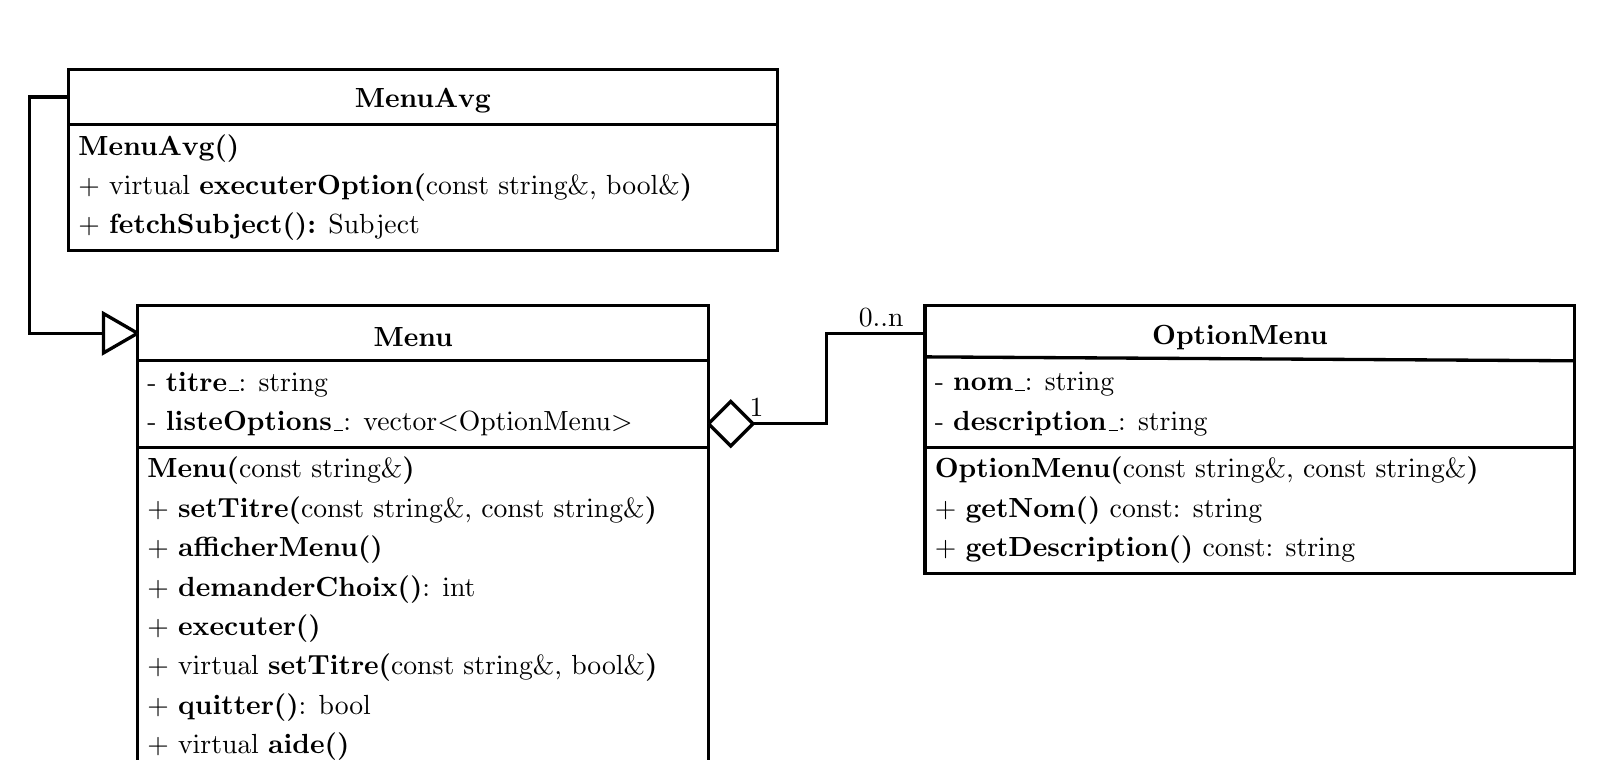
\begin{tikzpicture}[]
                \begin{scope}[xshift=10cm,yshift=-5cm]

                    \draw[very thick] (0,0.5) rectangle (8.25,-2.9);

                    \node[] at (4,0.1) {\textbf{OptionMenu}};
                    \node[anchor=west] at (0,-0.5) {- \textbf{nom\_}: string};
                    \node[anchor=west] at (0,-1) {- \textbf{description\_}: string};
                    \node[anchor=west] at (0,-1.6) {\textbf{OptionMenu(}const string\&, const string\&\textbf{)}};
                    \node[anchor=west] at (0,-2.1) {+ \textbf{getNom()} const: string};
                    \node[anchor=west] at (0,-2.6) {+ \textbf{getDescription()} const: string};
                    \draw[very thick] (0,-0.15) -- (8.25,-0.2);
                    \draw[very thick] (0,-1.3) -- (8.25,-1.3);
                \end{scope}
                \begin{scope}[yshift=-5cm]
                    \node[] at (3.5,0.1) {\textbf{Menu}};
                    \node[anchor=west] at (0,-0.5) {- \textbf{titre\_}: string};
                    \node[anchor=west] at (0,-1) {- \textbf{listeOptions\_}: vector$<$OptionMenu$>$};
                    \node[anchor=west] at (0,-1.6) {\textbf{Menu(}const string\&\textbf{)}};
                    \node[anchor=west] at (0,-2.1) {+ \textbf{setTitre(}const string\&, const string\&\textbf{)}};
                    \node[anchor=west] at (0,-2.6) {+ \textbf{afficherMenu()}};
                    \node[anchor=west] at (0,-3.1) {+ \textbf{demanderChoix()}: int};
                    \node[anchor=west] at (0,-3.6) {+ \textbf{executer()}};
                    \node[anchor=west] at (0,-4.1) {+ virtual \textbf{setTitre(}const string\&, bool\&\textbf{)}};
                    \node[anchor=west] at (0,-4.6) {+ \textbf{quitter()}: bool};
                    \node[anchor=west] at (0,-5.1) {+ virtual \textbf{aide()}};
                    \draw[very thick] (0,-1.3) -- (7.25,-1.3);
                    \draw[very thick] (0,-0.2) -- (7.25,-0.2);
                    \draw[very thick] (0,0.5) rectangle (7.25,-5.4);
                \end{scope}

                \begin{scope}[xshift=-0.875cm, yshift=-2cm]
                    \node[] at (4.5,0.1) {\textbf{MenuAvg}};
                    \node[anchor=west] at (0,-0.5) {\textbf{MenuAvg()}};
                    \node[anchor=west] at (0,-1) {+ virtual \textbf{executerOption(}const string\&, bool\&\textbf{)}};
                    \node[anchor=west] at (0,-1.5) {+ \textbf{fetchSubject():} Subject};
                    \draw[very thick] (0,0.5) rectangle (9,-1.8);
                    \draw[very thick] (0,-0.2) -- (9,-0.2);


                \end{scope}

                \draw[very thick](-0.875,-1.85) -- ++ (-0.5,0) |- (0,-4.85) coordinate (menu);

                \filldraw[fill=white, very thick] (menu) -- ++ (150:0.5) -- ++ (0,-0.5) -- ++ (30:0.5);

                \draw[very thick](7.25,-6) coordinate(menuopt)-- ++ (1.5,0) |- (10,-4.85) coordinate (option);

                \filldraw[fill=white,very thick] (menuopt) -- ++ (45:0.4) -- ++ (-45:0.4) -- ++ (-135:0.4) -- ++ (135:0.4);

                \node[above=0.2cm,left=0.15cm] at (option) {0..n};
                \node[above=0.2cm,right=0.4cm] at (menuopt) {1};



            \end{tikzpicture}
        }
    }
\end{figure}


\end{document}